\documentclass[]{beamer}
%%\documentclass[notes]{beamer}
\usepackage{etex}



%% Default will be false for \handouts; it can be set to true within
%% the Makefile.

\newcommand{\adv}{{\tiny (Advanced)}}

\usepackage{showexpl,xspace}
\usepackage{ifthen}
\usepackage{amsmath}
\usepackage{xspace}
\usepackage{xskak}

\providecommand*{\latex}{\LaTeX\xspace}

\providecommand*{\handouts}{false}

\ifthenelse{\equal{\handouts}{true}}
{\usepackage{pgfpages}
  \pgfpagesuselayout{4 on 1}[a4paper,landscape]}
{}
%% Handling handouts: end %%%%%%%%%%%%%%%%%%%%%%%%%%%%%%%%%%%%%%%%%%%%%%





%% \newcommand{\pauseb}{}

%% fragwidth will measure the width of the text, and then we use
%% it for the width of the textblock.
\newdimen{\fragwidth}

\newcommand{\mybottomleft}[1]{
\settowidth{\fragwidth}{#1}
\begin{textblock*}{\fragwidth}[0,0](2mm,90mm)  %% {width}(horiz, vert)
  #1
\end{textblock*}
}

\newcommand{\mybottomright}[1]{
\settowidth{\fragwidth}{#1}
\begin{textblock*}{\fragwidth}[1,0](126mm,90mm)  %% {width}(horiz, vert)
  #1
\end{textblock*}
}

\usepackage{graphicx}

\def\0{\hbox{\phantom{\footnotesize\rm 0}}}

%% Seek help from beamer crowd about this?
\makeatletter
\def\DIfF^#1{%
  \mathop{\mathrm{\mathstrut \text{d}}}%
  \nolimits^{#1}\gobblespace}
\makeatother

%% This snippet is from the TeX faq and allows us to use \maxwidth
%% for the max size of an image.
\makeatletter
\def\maxwidth{%
  \ifdim\Gin@nat@width>\linewidth
  \linewidth
  \else
  \Gin@nat@width
  \fi
}
\makeatother
\usepackage[overlay]{textpos}

\mode<presentation>
{
  \setbeamersize{text margin left=0.25cm}
  \setbeamersize{text margin right=0.25cm}

  \beamertemplatedotitem

  \beamertemplateheadempty %% Remove headline (at top of frame)
  %% \beamertemplatefootempty %% Remove headline (at top of frame)
  %% \beamertemplatefootpagenumber %% page number only in footer.
  %% Remove navigation icons.
  \setbeamertemplate{navigation symbols}{}

  %% Show start of every lecture. Not available in article.
  \AtBeginLecture{\frame{\Large Lecture \insertlecture}}
}




\title{\LaTeX\ 101}
\author{Stephen J. Eglen}


\institute{Cambridge Computational Biology Institute\\
  Department of Applied Mathematics and Theoretical Physics\\
  University of Cambridge\\
  \url{http://www.damtp.cam.ac.uk/user/eglen/teaching/latex}
}

\date{October 2014}

\begin{document}

\begin{frame}
  \titlepage
\end{frame}

\begin{frame}
  \frametitle{What is \LaTeX?}
  \begin{itemize}
  \item Typesetting, not WYSIWYG.
  \item Given a source file (file.tex) you \textbf{compile} your document (file.pdf).
  \item Heavily used by mathematicians/scientists/publishers for
    formatting papers/books.
  \item Logical markup of your document (like HTML) rather than
    specifying exactly how you want it look.
  \item Use Word (or program of your choice) if you want to.

  \item These slides are written in \latex using the ``beamer'' package.

  \item You can typeset music, wiring diagrams, chess \ldots

  \end{itemize}
\end{frame}

\begin{frame}[fragile]
  %% \frametitle{Chess}
  %% This uses the xskak package.  "skak" is "chess" in Danish.
  %% Example taken from http://mirror.ox.ac.uk/sites/ctan.org/macros/latex/contrib/xskak/xskak.pdf
  \begin{LTXexample}[pos=b,rframe={}]
    \newchessgame  % from the xskak package
    \mainline{1. e4 e5 2. Nf3 Nc6 3. Bb5 a6 4. Ba4 Nf6}
    \chessboard
  \end{LTXexample}
\end{frame}


\begin{frame}[fragile]
  \frametitle{``Hello world'' example}

  \section*{hi there}
  \begin{LTXexample}[pos=b,rframe={}]
\documentclass{article}
\begin{document}
  Hello world.  Welcome to \LaTeX.
\end{document}
\end{LTXexample}
%% Complicated begin/end documents don't work in beamer.
%% http://tex.stackexchange.com/questions/6006/how-to-use-showexpl-with-an-external-class
\end{frame}


\begin{frame}[fragile]
  \frametitle{Another example {\tiny (Taken from \url{showexpl-test.tex})}}
  \begin{LTXexample}[pos=b,wide,width=.65,preset=\LARGE,rframe={}]
\documentclass[a4paper,twoside]{article}
\begin{document}
\begin{equation}
  \sigma(t)=\frac{1}{\sqrt{2\pi}}
  \int^t_0 e^{-x^2/2} dx 
\end{equation}
\end{document}
\end{LTXexample}

\end{frame}

\begin{frame}
  \frametitle{Getting started}

  \begin{itemize}
  \item   \latex is free to download.  

  \item   Can use it from the command line.

  \item  Lots of editors/GUIs available.

  \item I suggest trying \textit{texstudio} or \textit{texmaker}.
    They both handle all the compilation steps for you and provides
    easy way of forward/inverse searching (Ctrl + left mouse button).

  \item \url{http://www.lyx.org} = latex engine + WYSIWYG interface.
  \end{itemize}

\end{frame}

\begin{frame}[fragile]
  \frametitle{Welcome to the 21st century}

  \begin{enumerate}
  \item   Many \latex guides describe how you can create .dvi files and .ps
    (postscript) files.  
  \item   Ignore that; we typically create .pdf files now, via
    'pdflatex'.
  \item   Create your figures in .pdf or .eps wherever you can, else
    png/jpg.

  \item Matlab users: .eps files have tight bounding boxes, whereas
    pdf files do not.  However, pdflatex will silently convert \url{sin.eps} to
    \url{sin-eps-converted-to.pdf} for you:
    \begin{verbatim}
    \fbox{\includegraphics[width=6cm]{sin.eps}}
    \end{verbatim}
  \end{enumerate}
\end{frame}



\begin{frame}[fragile]
  \frametitle{\latex syntax - commands}

  \begin{itemize}
  \item \latex commands start with backslash and are case-sensitive:

    \begin{LTXexample}[pos=b]
      The \large cat \LARGE sat on \Huge the \normalsize mat
    \end{LTXexample}

    \item Commands can take compulsory \{ \ldots \} and optional [
      \ldots ] arguments.
      \begin{LTXexample}[pos=b]
        A \rule{10mm}{3mm}  B \rule[-1mm]{10mm}{3mm}  
      \end{LTXexample}
    \item You can sometimes drop \{ and \}:
      \begin{LTXexample}[pos=b]
        e.g. if superscript is one character: compare $x^3$ with
        $x^{19}$ and with $x^19$.

      \end{LTXexample}
  \end{itemize}
\end{frame}


\begin{frame}[fragile]
  \frametitle{Special characters}

Some characters are commands.  To type these characters, you normally
escape them:
\begin{LTXexample}[pos=b]
  I got a 30\% discount, saving me a few \$\$\$ \ldots
\end{LTXexample}

The most common characters that need escaping are:
\begin{center}
\verb+\ $ ^ _ % # & ~ { } +
\end{center}

\end{frame}

\begin{frame}[fragile]
  \frametitle{Space}
  

  \begin{LTXexample}[pos=b]
Multiple   spaces   between words are treated as 
one space.  

Blank lines denote
paragraph separators.

Use a non-breaking space, like 3~mm, to prevent line-breaks.  Even
better for separating numbers from units, try a small non-breaking
space, e.g. 3\,mm.
  \end{LTXexample}
\end{frame}





\begin{frame}[fragile]
  \frametitle{Environments}

An environment is a block of latex code to provide some
functionality.  They can be nested.
\begin{LTXexample}[pos=r]
  \textbf{Top TV programmes}:
  \begin{enumerate}
  \item Homeland
  \item The West Wing
    \begin{itemize}
    \item Series 1
    \item (Not series 3)
    \end{itemize}
  \item 24
  \end{enumerate}
\end{LTXexample}
\end{frame}



\begin{frame}[fragile]
  \frametitle{Typesetting math}

  \begin{enumerate}
  \item \latex normally is in text mode.  You must switch to math mode
    using \$ to get into and out of math.
\begin{LTXexample}[pos=b]
  This equation $x^2 + y^2 = z^2$ is in-line; compare with:
  \begin{eqnarray}
    \label{eq:key}
    I_1 &= \int_0^{2 \pi} \sin (x^2) dx \nonumber \\
    \text{but}\, I_2 &= \int_0^{2 \pi} \cos (x^2) dx \label{key}
  \end{eqnarray}
  The dx in Equation \ref{key} needs fixing later \ldots
\end{LTXexample}
    
  \end{enumerate}
\end{frame}


\begin{frame}
  \frametitle{amsmath -- AMS mathematical facilities for \latex}

  \url{http://mirrors.ctan.org/macros/latex/required/amslatex/math/amsldoc.pdf}

  Lots of good examples for formatting maths.  See the examples in:

  \url{http://mirrors.ctan.org/macros/latex/required/amslatex/math/testmath.pdf}

  \vspace*{1cm}

  This is an example of a package that has been contributed to
  \latex.  These packages are available on Comprehensive TeX Archive
  Network (CTAN).  Most of them are downloaded for you when installed \latex.
\end{frame}
\begin{frame}
  \frametitle{Universe of mathematics symbols and operators}


  \url{http://mirror.ox.ac.uk/sites/ctan.org/info/symbols/comprehensive/symbols-a4.pdf}

  contains $\sim$6000 symbols and \latex commands to
  generate them.  e.g. see Table 97 for inequalities:

  \centerline{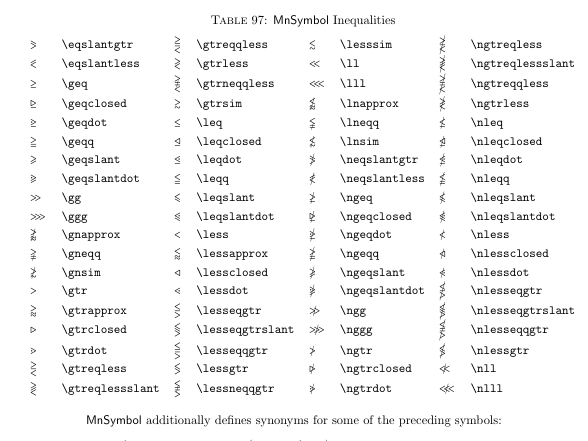
\includegraphics[width=9cm]{table97-a4symbols.png}}


\end{frame}

\begin{frame}
  \frametitle{Finding maths operators the ``modern'' way}

  \begin{itemize}
  \item Draw some equations and it will try to render it in latex or
    mathml:

    Wolfram: graph an equation, with latex output.
    \url{http://webdemo.myscript.com/\#/demo/equation}
    %% needed to escape hash

  \item http://detexify.kirelabs.org/classify.html



  \end{itemize}



\end{frame}


\begin{frame}[fragile]
  \frametitle{Defining your own commands}


  \begin{LTXexample}[pos=b]
    \newcommand{\betaIIKO}
    {\ensuremath{\beta\mathit{2}^{-/-}}\xspace}
    The \betaIIKO mouse is widely studied \ldots 
    the \betaIIKO command  is easier for me
    to type than the whole expansion.

    \newcommand{\nnn}[1]{\ensuremath{#1^{#1^{#1}}}}
    Or we can compare \nnn{3} with \nnn{16}.
  \end{LTXexample}

\textit{Typesetting mathematics for science} has many hints for
getting things ``just right'', e.g. the differential operator, partial, total derivatives:
\url{http://www.tug.org/TUGboat/Articles/tb18-1/tb54becc.pdf}


\end{frame}


\begin{frame}[fragile]
  \frametitle{Bibliography / citations}

Entries like the following are stored in a bibliography file:

\begin{verbatim}
@article{ihaka1996,
  author =    {R. Ihaka and R. Gentleman},
  title =     {R: A Language for Data Analysis and Graphics},
  journal =   {Journal of Computational . . . Statistics},
  year =      1996,
  volume =    5,
  pages =     {299--314}
}
\end{verbatim}

which you can then cite using e.g.
\begin{verbatim}
We used the R programming environment \cite{ihaka1996}
for our analysis.
\end{verbatim}

To create:


\begin{verbatim}
We used the R programming environment (Ihaka and Gentleman, 
1996) for our analysis.
\end{verbatim}

and references at end.  See \url{texintro/intro.tex}
for more info.


\end{frame}

\begin{frame}
  \frametitle{Creating a bibliography}

  \begin{itemize}
  \item Create it by hand.  Slow, tedious, and error-prone.
  \item Grab them from Google scholar, e.g. 
    \url{http://scholar.google.co.uk/scholar?q=ihaka+gentleman}.  The
    cite link takes you to the formats for citing (you may need to
    configure google scholar).
  \item zotero/paperpile/mendeley all generate good bibtex
    entries.
    
  \end{itemize}


\end{frame}




\begin{frame}[fragile]
  \frametitle{Preamble}

  \begin{enumerate}
  \item Everything before the \verb+begin{document}+ is the preamble.
  \item Use it to set up document, load packages.  My favourite
    packages:


\begin{verbatim}
\usepackage{graphicx}           % Including graphics.
\usepackage{url}                % active URLs.
\usepackage[a4paper,margin=2cm]{geometry}
\usepackage{mathpazo}           % or mathptmx
\usepackage{amsmath}            % AMS Maths goodies
\end{verbatim}
  \end{enumerate}
\end{frame}


\begin{frame}
  \frametitle{Your choice of fonts}

  Choose a font that has good support for both math and text modes:

  \begin{enumerate}
  \item Do nothing.  Stick with Donald Knuth's \textit{Computer Modern}.  
  \item I prefer mathpazo (Palatino) or mathptmx (Times).
  \item Explore the free guide \url{http://mirrors.ctan.org/info/Free_Math_Font_Survey/en/survey.html}
  \end{enumerate}
\end{frame}


\begin{frame}
  \frametitle{Floats: tables and figures}

  \begin{itemize}
  \item Floats are objects (tables, figures) that move in your
    document; \latex will move them to somewhere it thinks sensible.
  \item If you don't like where it put a float, relax.  You can give
    it hints, but normally it does a good job.  


  \item This is the \latex philosophy in general -- let it worry about
    layout so that you worry about content.
  \item You can then refer to figures/tables by labels.
  \end{itemize}
\end{frame}

\begin{frame}[fragile]
  \frametitle{Tables}

  \begin{LTXexample}[pos=b,rframe={}]
\begin{table}
  \centering
  \begin{tabular}{|l|rr|}  \hline
    year & min temp (C) & max temp (C)\\ \hline
    1970 & -5 & 35\\
    1980 & -3 & 30\\
    1985 & -2 & 32\\ \hline
  \end{tabular}
  \caption{Fictional min/max temperatures.} \label{tab:simple}
\end{table}
  \end{LTXexample}
\end{frame}


\begin{frame}[fragile]
  \frametitle{Labels and references}
  \label{labels}
  \begin{enumerate}
  \item For complex documents, rather than writing ``Table 3'', it is
    better to give the Table a label using \verb+\label{results}+, and then refer to that label,
      using e.g. \verb+See Table~\ref{results}+.  

      \item You can also refer to figures, equations, sections in a
        similar way.  

        \item To refer to pages you can do:
          \begin{LTXexample}[pos=b]
            This is on page \pageref{labels}.
          \end{LTXexample}
  \end{enumerate}
\end{frame}

\begin{frame}[fragile]
  \frametitle{Figures}

  \begin{LTXexample}[pos=b,rframe={}]
\begin{figure}
  \centering
  \fbox{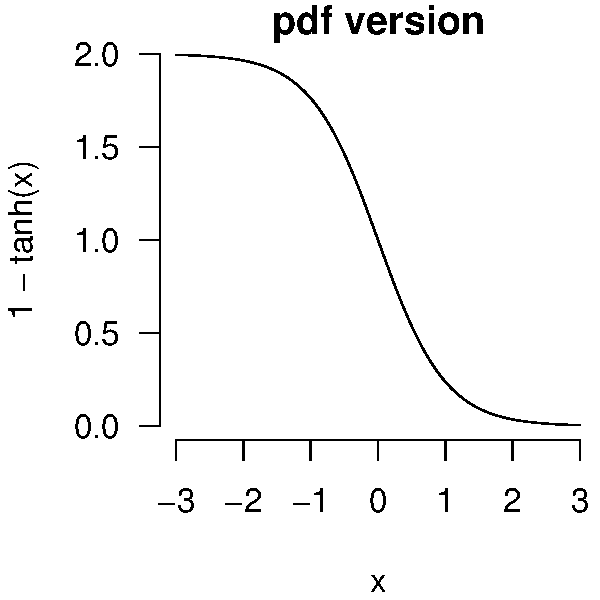
\includegraphics[width=4cm]{sigmoid}}
  \caption{Example of a sigmoidal curve.}
  \label{fig:example}
\end{figure}
  \end{LTXexample}

Looks for file in current directory (or you can keep a path of figures).
\end{frame}



\begin{frame}
  \frametitle{Advanced topics}

  \begin{description}

  \item[mathml] \url{http://docs.mathjax.org/en/latest/tex.html} 
    latex in your web pages is converted to mathml, and then rendered.
  \item[lualatex] Embedded programming language (LUA) within latex.
  \item[Reproducible research] 
  \url{https://github.com/sje30/waverepo/blob/master/paper/waverepo_paper.Rnw}
  \url{http://www.gigasciencejournal.com/content/3/1/3}

\item[markdown] If latex looks too cumbersome/heavyweight, write in
  markdown, which can then be converted to .tex (.pdf) or .html or
  .doc by \url{http://johnmacfarlane.net/pandoc/}
    
  \end{description}

\end{frame}


\begin{frame}
  \frametitle{Getting help}
  \begin{enumerate}

  \item Work through Lamport's book slowly and surely.
    
  \item Google what you need to.  Often you can find good answers on
    \url{http://tex.stackexchange.com/}

  \item Keep it simple for now!  Focus on the content, not the form.

  \item \textit{The \latex companion} lists vast number of packages.
  \end{enumerate}
\end{frame}


\begin{frame}
  \frametitle{Further reading}

Lamport (1994) LATEX: a Document Preparation System : User’s Guide
and Reference Manual.

Kopka and Daly (2003) A Guide to LATEX (Tools and Techniques for
Computer Typesetting).

Mittelbach  et al. (2004.) The Latex Companion.

\vspace*{3cm}

\textbf{Acknowledgements} Thanks to Robert Stojnic and Markus Kuhn, who wrote
similar lectures and shared material.

\end{frame}


\begin{frame}
  \frametitle{History of \TeX \xspace  and \latex}
  
  \TeX\xspace was originally a six-month project in 1978 started by
  Donald Knuth, which took ten years:
  
  \url{http://www.ctan.org/ctan-portal/tex/}
\end{frame}

\begin{frame}
  \frametitle{Command line material \adv }

  If you run from the command line, you need to follow instructions on
  how often to re-rerun \latex to resolve references.

  latexmk, texi2pdf help with this problem.

\end{frame}


\end{document}

% LocalWords:  Eglen 

